%!TEX root = main.tex

\begin{center}
\textbf{ВВЕДЕНИЕ}
\end{center}
\addcontentsline{toc}{section}{ВВЕДЕНИЕ}

Теория автоматов --- самостоятельный раздел математики, имеющий разнообразную проблематику и приложения.  Основными понятиями теории автоматов являются понятия абстрактного автомата и понятие композиции автоматов. Эти понятия являются разумными абстракциями реально существующих дискретных устройств --- автоматов. Понятие абстрактного автомата позволяет характеризовать устройство с точки зрения алгоритма его функционирования, т.е. алгоритма переработки информации, который оно реализует. Понятие композиции автоматов позволяет характеризовать устройство с точки зрения его структуры, иными словами, даёт представление, каким образом данное устройство построено из других, более элементарных.

Академик В.М. Глушков показал, что любое устройство обработки цифровой информации можно представить в виде совокупности двух взаимодействующих автоматов --- управляющего УА и операционного ОА (Рисунок \ref{figure:intro_pic}).

\begin{figure}[H]
	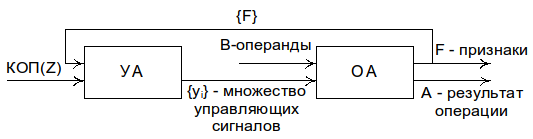
\includegraphics[scale=0.6]{images/intro.png}
	\caption{Структура цифрового автомата}
	\label{figure:intro_pic}
\end{figure}

ОА осуществляет непосредственную обработку данных путем выполнения элементарных операций над словами и выдает результат преобразования в виде двух слов: $A$ (результат) и $F$ (признаки результата, т.е. сигналы о знаках и особых значениях промежуточных и конечных результатов операций). Выполнение элементарных операций инициируется соответствующими управляющими сигналами {$y_0, y_1, y_2 ... y_m$}, которые формируются УА. 

В курсовой работе требуется разработать ОА, реализующий заданный набор арифметико-логических операций.
